\section{Electronics Design}

\subsection{Computers}

\subsubsection{Main Computer}

Nearly all computation is performed on a single laptop containing a quadcore Intel Core i7 CPU,
CUDA enabled NVIDIA 285M GPU, and 6 GB of RAM. This computer is responsible for all vision,
LIDAR, and GPS data processing and all path planning and control algorithms. It also forms 
the core of the sensor interconnects, providing the firewire and USB bus which the camera, GPS, and
microcontrollers use.

\subsubsection{MCU}

This year saw a drastic reduction in the number of microcontrollers used. While last year's design utilized 6 Arduino Duemilanove boards to accomplish the task of interfacing with the the motors and encoders, this year's design was able to accomplish the same task while utilizing only a single Arduino Uno board. This was made possible through the design of a custom interfacing daughterboard.

\begin{figure}[H]
\begin{center}
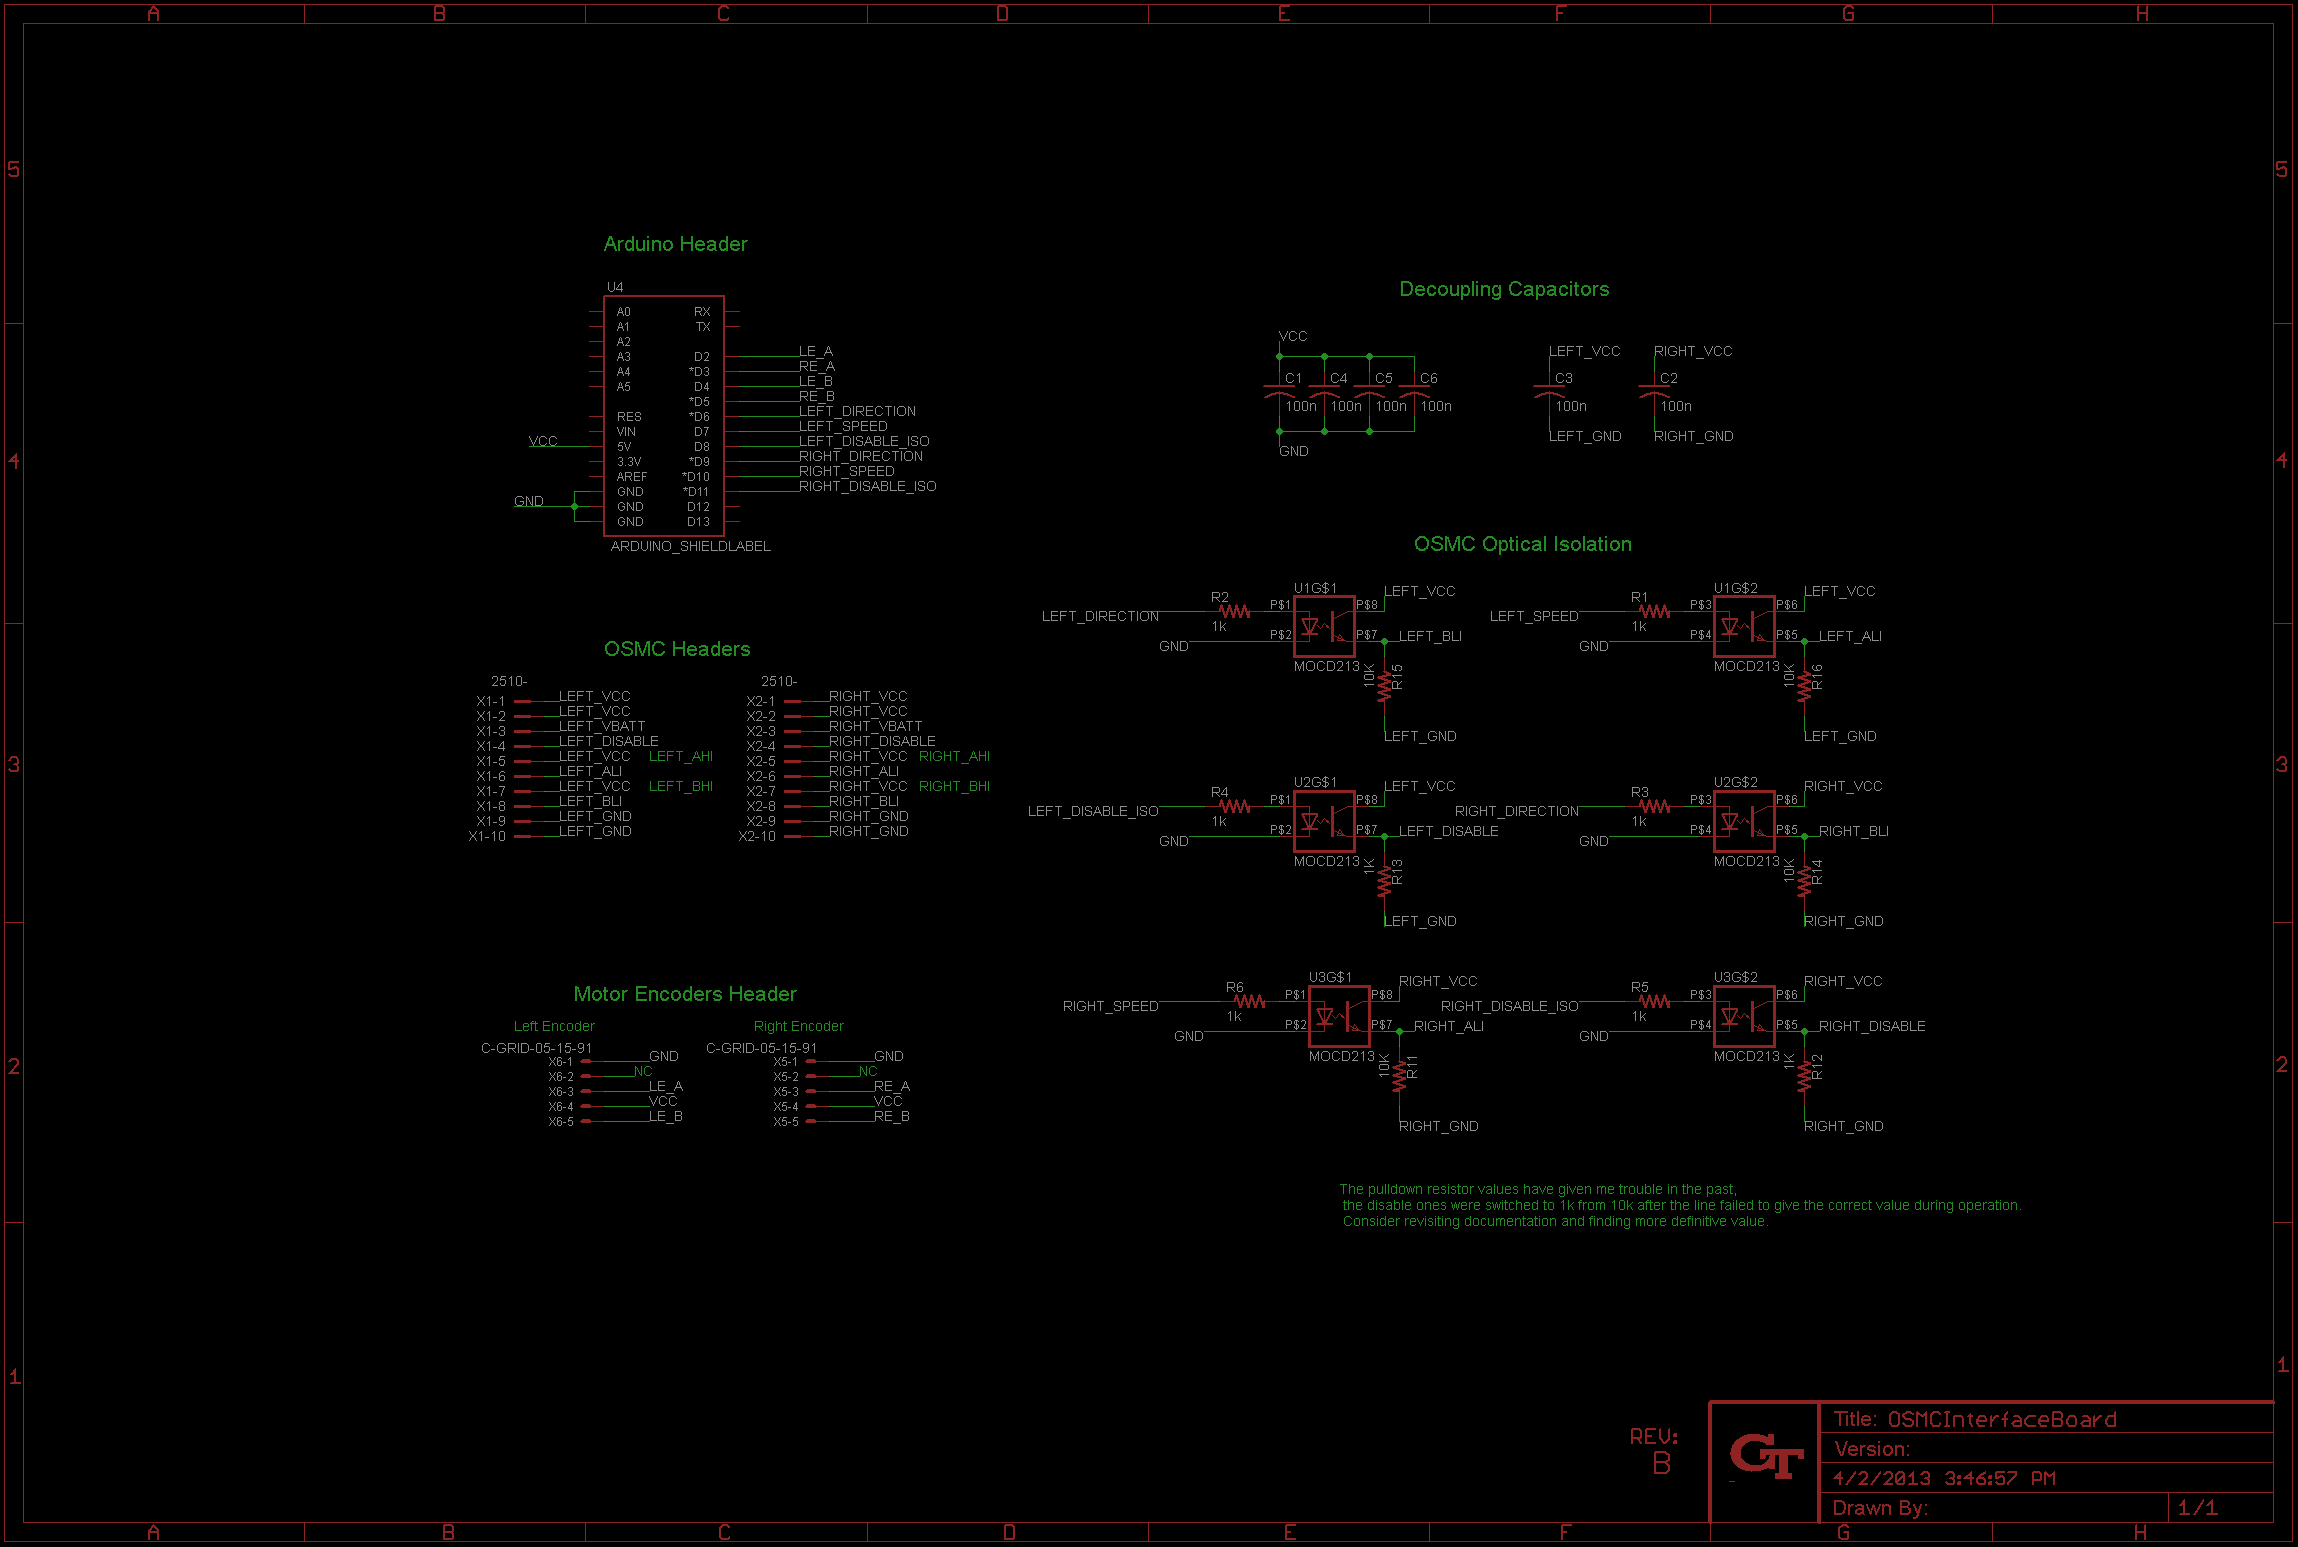
\includegraphics[width=5in]{./Pics/schematisch.png}
\caption{Electrical Board Schematic}
\label{FIG:Schematic}
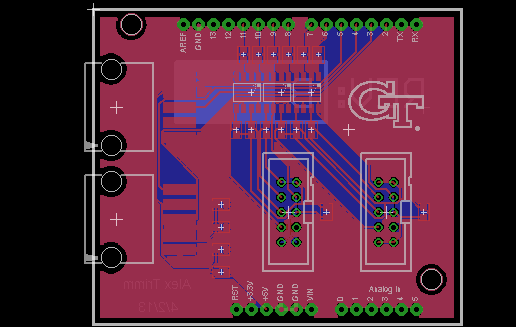
\includegraphics[width=3in]{./Pics/baord.png}
\caption{Daughter Board}
\label{FIG:Board}
\end{center}
\end{figure}


\subsection{Sensors}

This year saw a significant additions to the existing sensor system. These included the addition of an ArduPilot IMU and a BumbleBee2 Stereo Camera. Additionally, the new mechanical design led to several changes in the existing sensor system.

\subsubsection{LIDAR}

Misti employs a Sick NAV200 LIDAR to provide convenient and straightforward obstacle detection. The LIDAR has a $270^{\circ}$ FOV and a 10 meter range.

\subsubsection{Stereo Camera}

Misti will be the first Georgia Tech IGVC robot to utilize a stereo camera. The stereo camera chosen is a Bumblebee 2 made by Point Grey Technologies. This camera delivers two 1024x768 images at 20 fps. The camera uses a Firewire connection to interface with the main laptop. 

\subsubsection{GPS}

A GPS is used to provide world position to the robot, allowing obstacles to be placed in world space and allowing waypoints to be followed. A Hemisphere A100 Smart Antenna GPS is mounted to the mast to allow a clear view of the sky. This GPS is accurate to $<2.5$ m / $<.6$ m (GPS / WAAS) and has a ``time to first fix" of less than one second. The GPS updates 20 times per second.

\subsubsection{IMU}

Misti also utilize an ArduPilot IMU. This IMU includes a 3-axis accelerometer, 3-axis gyroscope and a 3-axis magnetometer as well as a barometric pressure sensor. The board contains an ATmega2560 chip and can both be programmed and communicate with the main computer through a USB connection.
 
\subsubsection{Encoders}

Each gearbox is connected to a quadrature wheel encoder, allowing wheel rate and absolute distance to be measured. This allows the velocity of the robot to be measured, as well as the distance the robot has travelled. The encoder is a US Digital E3, with 200 counts per revolution and an index channel. This allows for wheel rates to be sensed. One quadrature line from each encoder is connected to an interrupt pin on the microcontroller, which then feeds the state of the lines to a state machine which increments or decrements a wheel counter.

\subsection {Power}

\subsubsection{Sources}
Main power for the robot comes from two deep-cycle lead acid gell-cell batteries. These batteries are
 connected in series to produce a nominal 24 VDC supply. These batteries each provide 48 Amp-Hours of energy, making the robot's total capacity 1052 Watt-Hours. This increased capacity over previous designs counteracts the increased mass of Misti over her predecessor and leaves the total estimated runtime approximately 1 hour of driving.

\subsubsection{Distribution}
The batteries are connected to a power distribution board, which allows the connection to each
motor to be fused with a limit of 40 Amps, allowing power to be cut in the event of a motor stall 
to prevent damage to the H-bridge and motor. Each motor is connected to two OSMC H-bridges, which allow the motors to be driven from the Arduino microcontroller. Each OSMC is capable of switching up to 50 VDC at 160A cont / 300A peak, allowing significant margin above our standard operating power of around 24 VDC / 20 A. 

Power is also provided to several DC-DC buck converters, which output 5 VDC, 12 VDC, and 19.5 VDC for the other electronics on the robot.

\begin{figure}[H]
\begin{center}
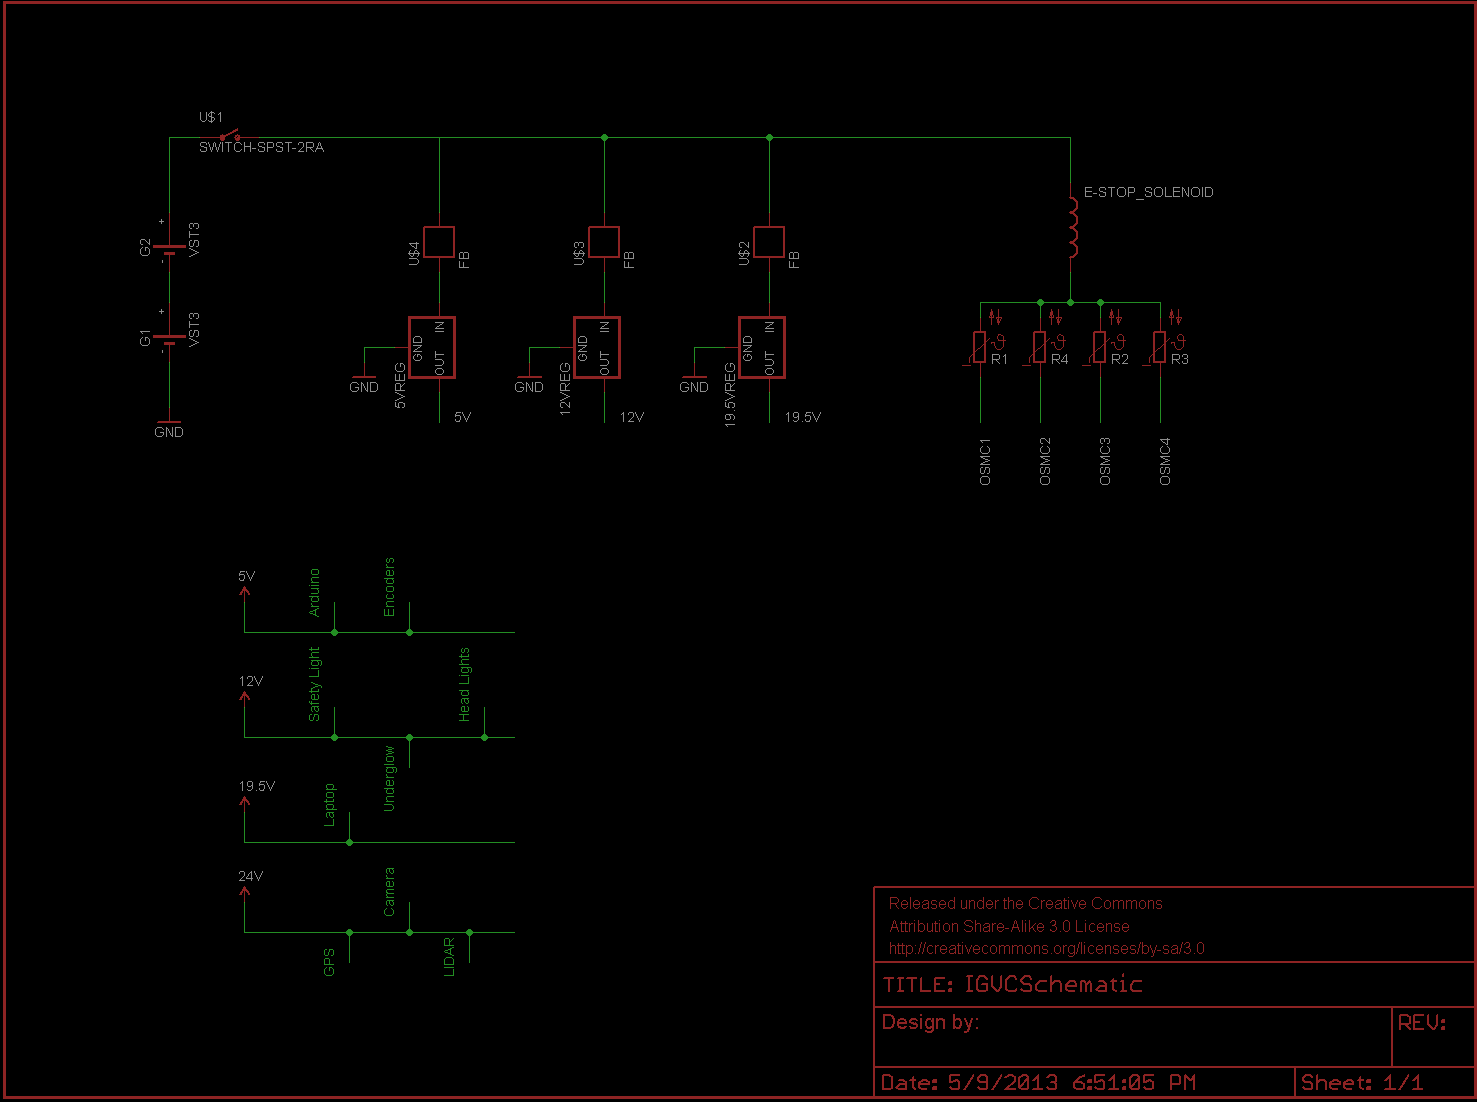
\includegraphics[width=5in]{./Pics/PowerSchematic.png}
\caption{Power Distribution Schematic}
\label{FIG:Distribution}
\end{center}
\end{figure}
